\documentclass[aspectratio=169,xcolor=table,10pt, notes=hide]{beamer}


\usetheme[faculty=phil]{fibeamer}
\usepackage{polyglossia}

\setmainlanguage{russian} %% main locale instead of `english`, you
%% can typeset the presentation in either Czech or Slovak,
%% respectively.
\setotherlanguages{english} %% The additional keys allow
%%
%%   \begin{otherlanguage}{czech}   ... \end{otherlanguage}
%%   \begin{otherlanguage}{slovak}  ... \end{otherlanguage}
%%
%% These macros specify information about the presentation
\title[Theoretical Mechanics]{Theoretical Mechanics, Lab 1: KIN PART} %% that will be typeset on the
\subtitle{Intro \\ Linear Algebra recap \\ Particle kinematics } %% title page.
\author{Oleg Bulichev}
%% These additional packages are used within the document:
\usepackage{ragged2e}  % `\justifying` text
\usepackage{booktabs}  % Tables
\usepackage{tabularx}
\usepackage{tikz}      % Diagrams
\usetikzlibrary{decorations.pathreplacing,calligraphy,calc,graphs, shapes, backgrounds}
\usepackage{amsmath, amssymb}
\usepackage{url}       % `\url`s
\usepackage{listings}  % Code listings
\usepackage{floatrow}
\usepackage{mathtools}
\usepackage{fontspec}
\usepackage{multicol}
\usepackage{pdfpages}
\usepackage{wrapfig}
\usepackage{animate}
\usepackage{booktabs}
\usepackage{multirow}
\usepackage{multimedia}
\usepackage{makecell}
\usepackage{colortbl}
\usepackage{hhline}
\usepackage{rotating}
\usepackage{amsmath}

\usepackage[font={}, labelfont=it,textfont={it},justification=centering, skip=0pt]{caption}
% will apply to all subcaptions
\usepackage[font={},skip=2pt]{subcaption}


\graphicspath{{resources/}}
\frenchspacing




% \setbeamertemplate{caption}[numbered]
\captionsetup[figure]{labelformat=empty}


\newcommand{\fbckg}[1]{\usebackgroundtemplate{\includegraphics[width=\paperwidth]{#1}}}%frame background

\usepackage[framemethod=TikZ]{mdframed}
\newcommand{\dbox}[1]{
\begin{mdframed}[roundcorner=3pt, backgroundcolor=yellow, linewidth=0]
\vspace{1mm}
{#1}
\vspace{1mm}
\end{mdframed}
}
\addtobeamertemplate{frametitle}{}{\vspace{-0.35cm}}

% \usepackage{pgfpages}
% \pgfpagesuselayout{4 on 1}[a4paper,border shrink=2mm,landscape]
\usepackage{color}
\usepackage{rotating}
\usepackage{tabularray}

\begin{document}
\setlength{\abovedisplayskip}{0pt}
\setlength{\belowdisplayskip}{0pt}
\setlength{\abovedisplayshortskip}{0pt}
\setlength{\belowdisplayshortskip}{0pt}

\fbckg{fibeamer/figs/title_page.png}
\frame[c]{\setcounter{framenumber}{0}
    \usebeamerfont{title}%
    \usebeamercolor[fg]{title}%
    \begin{minipage}[b][6.3\baselineskip][b]{\textwidth}%
        \textcolor{black}{\raggedright\inserttitle}
    \end{minipage}
    % \vskip-1.5\baselineskip

    \usebeamerfont{subtitle}%
    \usebeamercolor[fg]{framesubtitle}%
    \begin{minipage}[b][3\baselineskip][b]{\textwidth}
        \raggedright%
        \insertsubtitle%
    \end{minipage}
    \vskip.25\baselineskip
}

\note{Рассказать про требования, как работаем сколько домашек итп
    Провести ревью линала (объяснить зачем нужно)

    Решить задачи с кинематикой точки (сказать, что первая домашка связана с этой темой будет)

    В начале класса обсудить соглашения со студентами (фишка Брауна). Я обычно таким образом с телефонами борюсь

    Решение задач переписать с помощью планшета (текст печатать, формулы от руки, картинки вставлять. Время на задачу уходит час
}

\fbckg{fibeamer/figs/common.png}

\section*{Intro}

\begin{frame}[t]{About me}
    \framesubtitle{}
    \begin{exampleblock}{Education}
        \begin{itemize}
            \item Bachelor --- Bauman University (BMSTU) (honor diploma) \\ \textbf{Topic:} Aim control development of mobile vehicle <<Plastun>>
            \item Master --- Innopolis University (IU), Robotics \\ \textbf{Topic:} Development of biomimetic centipede robot <<StriRus>>
            \item PhD --- Innopolis University (IU), Robotics. \textit{Defense}: Volgograd State Technical University (VSTU)  \\ \textbf{Topic:} Tactile perception method development for a mobile walking~robot
        \end{itemize}
    \end{exampleblock}
    \begin{alertblock}{Current jobs}
        \begin{itemize}
            \item Senior lecturer (AGLA 1,2; Mechanics and Machines; Theoretical Mechanics)
            \item Coach (\href{https://t.me/dich_trainings}{RAGE club channel}: Hiking, Folk Games, HEMA)
        \end{itemize}
    \end{alertblock}
\end{frame}

\fbckg{fibeamer/figs/text_page.png}
\begin{frame}[plain]{}
    \vfill
    \begin{center}
        \huge
        \centering
        Agreements among the group \\
        (for now)
    \end{center}
    \vfill
\end{frame}

\fbckg{fibeamer/figs/common.png}

\begin{frame}[t]{Books for labs}
    \framesubtitle{}
    \begin{figure}[H]
        \centering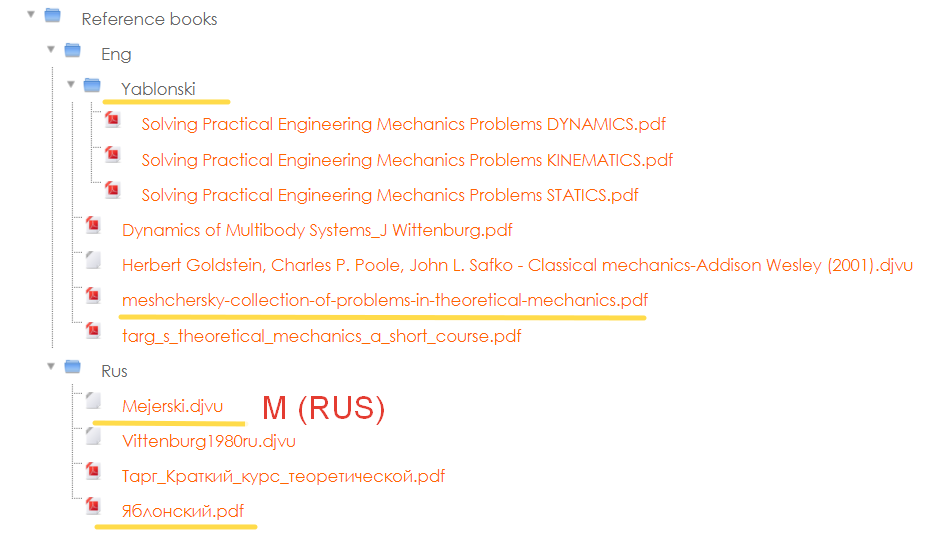
\includegraphics[height=6cm,width=1\textwidth,keepaspectratio]{image7.png}
    \end{figure}
\end{frame}

\begin{frame}[t]{Tasks goal}
    \framesubtitle{}
    \begin{enumerate}
        \item \textbf{Quizzes} — to check the understanding of the previous material.\\
              Starts in the beginning of the labs. Basic questions. \textit{Style guide formal criteria.}
        \item \textbf{Hometasks} — to depress you :) \textit{Style guide formal criteria + coding}.
        \begin{itemize}
            \item 6 weekly HWs. Will be given on \textbf{Wednesday}. 
            
            \textit{Deadline} --- Thursday, 9:00.
            \item 2 Big HWs. 2-3 weeks for solving. 
            
            \textit{Deadline} --- the day before midterm/final, 9:00.  
        \end{itemize}
    \end{enumerate}
\end{frame}


\begin{frame}[t]{Formal criteria}
    \framesubtitle{}
    \textbf{If you don’t follow formal criteria, you are losing 40\% of task grade score}
    \\For now:
    \begin{enumerate}
        \item Despite the paper sheet or digital, the answer should be \underline{highlighted}
    \end{enumerate}
\end{frame}

\begin{frame}[t]{Grading criteria}
    \framesubtitle{}
    \begin{itemize}
        \item[Qz:] Quizzes: 10\%: 5 best (2 \% each)
        \item[WHW:] Weekly HWs: 30 \% (5 \% each)
        \item[BHW:] Big HWs: 20\% (10 \% each) 
    \end{itemize}
    \textbf{Late policy:}
    \begin{itemize}
        \item WHWs --- no late policy. 0 score, if no data in Moodle. You can put a text file (\textbf{PDF}) with a link to Github, I wouldn't check the submission time, but if there are no solution --- 0 score.
        \item BHW 1 --- $-50\%$ on max grade for a task, BHW 2 --- no late policy.
    \end{itemize}
\end{frame}

\begin{frame}[c]{HW example: 2nd week}
    \framesubtitle{}
    \begin{figure}[H]
        \begin{subfigure}{0.49\textwidth}
            \centering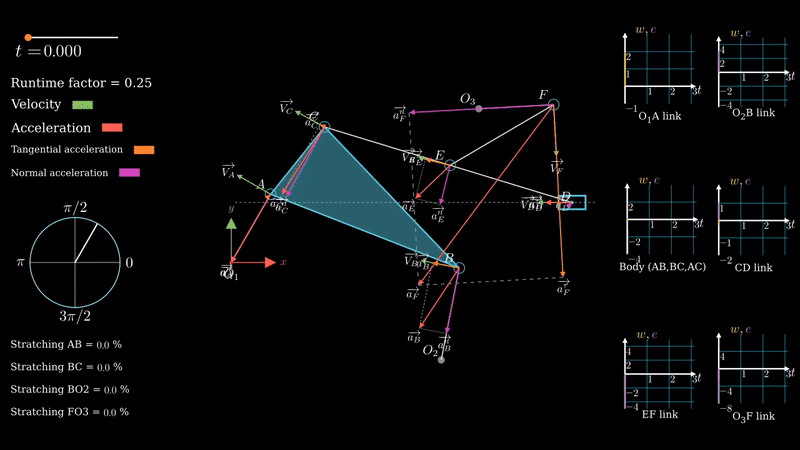
\includegraphics[height=6cm,width=1\textwidth,keepaspectratio]{image27.png}
        \end{subfigure}
        \begin{subfigure}{0.49\textwidth}
            \centering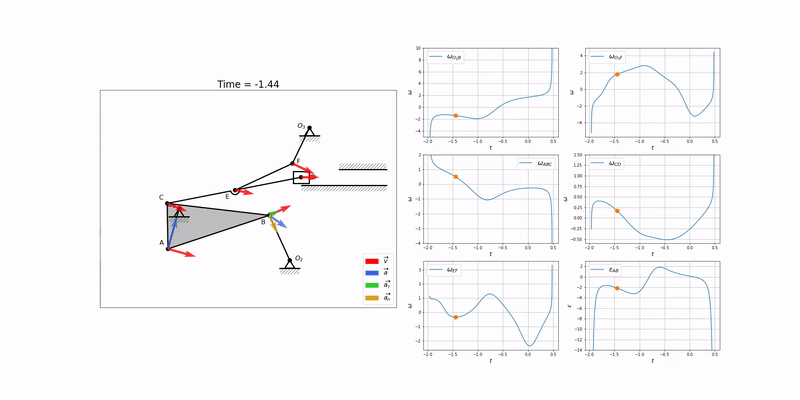
\includegraphics[height=6cm,width=1\textwidth,keepaspectratio]{image17.png}
        \end{subfigure}

    \end{figure}
\end{frame}

\begin{frame}[t]{Feedback from previous batch (1)
    }
    \framesubtitle{}
    \begin{figure}[H]
        \begin{subfigure}[b]{0.49\textwidth}
            \centering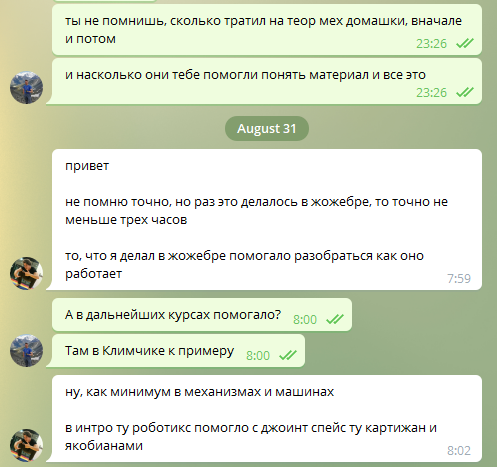
\includegraphics[height=6cm,width=1\textwidth,keepaspectratio]{image14.png}
        \end{subfigure}
        \begin{subfigure}[b]{0.49\textwidth}
            \centering
\includegraphics[height=6cm,width=0.8\textwidth,keepaspectratio]{image19.png}
            \centering
\includegraphics[height=6cm,width=0.8\textwidth,keepaspectratio]{image16.png}
        \end{subfigure}
    \end{figure}
\end{frame}

\begin{frame}[t]{Feedback from previous batch (2)}
    \framesubtitle{}
    \begin{figure}[H]
        \begin{subfigure}[b]{0.49\textwidth}
            \centering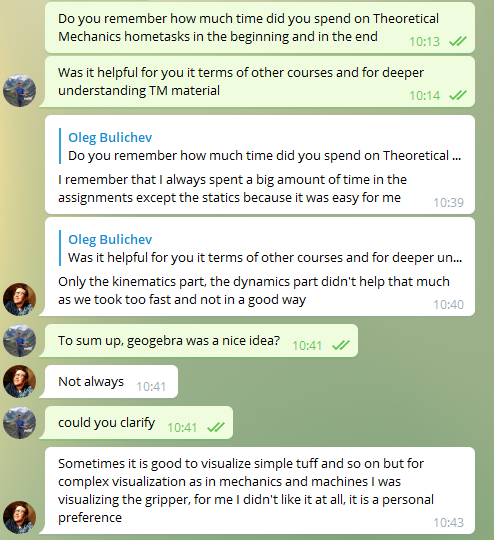
\includegraphics[height=6cm,width=1\textwidth,keepaspectratio]{image22.png}
        \end{subfigure}
        \begin{subfigure}[b]{0.49\textwidth}
            \centering
\includegraphics[height=6cm,width=1\textwidth,keepaspectratio]{image18.png}
            \centering
\includegraphics[height=6cm,width=1\textwidth,keepaspectratio]{image20.png}
        \end{subfigure}
    \end{figure}
\end{frame}

\begin{frame}[t]{Feedback from previous batch (3)
    }
    \framesubtitle{}
    \begin{figure}[H]
        \begin{subfigure}{0.49\textwidth}
            \centering
\includegraphics[height=6cm,width=1\textwidth,keepaspectratio]{image23.png}
        \end{subfigure}
        \begin{subfigure}{0.49\textwidth}
            \centering
\includegraphics[height=6cm,width=1\textwidth,keepaspectratio]{image21.png}
        \end{subfigure}
    \end{figure}
\end{frame}

\begin{frame}[t]{Tools for HWs and reports}
    \framesubtitle{}
    \textbf{Modeling} --- Python (Collab or Docker) / Matlab (Live Script) / Geogebra\\
    \textbf{Report} --- any tool (markdown, latex, word)

    \begin{center}
        \Large Report template will be given before the 1st HW.
    \end{center}
\end{frame}

\section*{AGLA recap}

\begin{frame}[t]{Cross product}
    \framesubtitle{Where it can be used}
    \begin{columns}[c,onlytextwidth]
        \begin{column}{0.49\textwidth}
            Relationship between \href{https://en.wikipedia.org/wiki/Force}{force} (F), \href{https://en.wikipedia.org/wiki/Torque}{torque}(τ), 
                \href{https://en.wikipedia.org/wiki/Momentum}{momentum} (p), and angular momentum 
                (L) vectors in a rotating system. r is the 
                \href{https://en.wikipedia.org/wiki/Position_(vector)}{position vector}  
        \end{column}
        \begin{column}{0.49\textwidth}
            \begin{figure}[H]
                \centering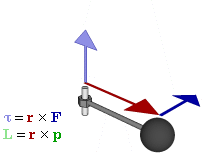
\includegraphics[height=6cm,width=1\textwidth,keepaspectratio]{../resources/image25.png}
            \end{figure}
        \end{column}
    \end{columns}
    \end{frame}
    
    \begin{frame}[t]{Cross product}
    \framesubtitle{How to calculate it: classical approach}
        \begin{figure}[H]
            \centering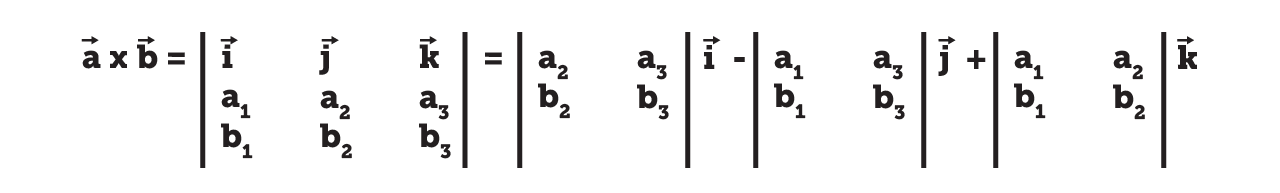
\includegraphics[height=6cm,width=1\textwidth,keepaspectratio]{image40.png}
            %\caption{caption_name}
            \label{fig:image40}
            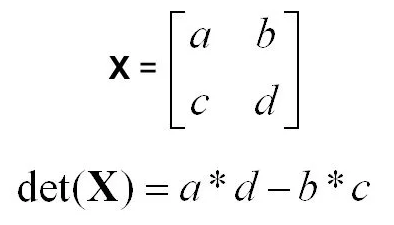
\includegraphics[height=6cm,width=0.3\textwidth,keepaspectratio]{image24.png}
            %\caption{caption_name}
            \label{fig:image24}
        \end{figure}
    \end{frame}
    
    \begin{frame}[t]{Cross product}
    \framesubtitle{How to calculate it: skew-symmetric matrix}
        \begin{figure}[H]
            \centering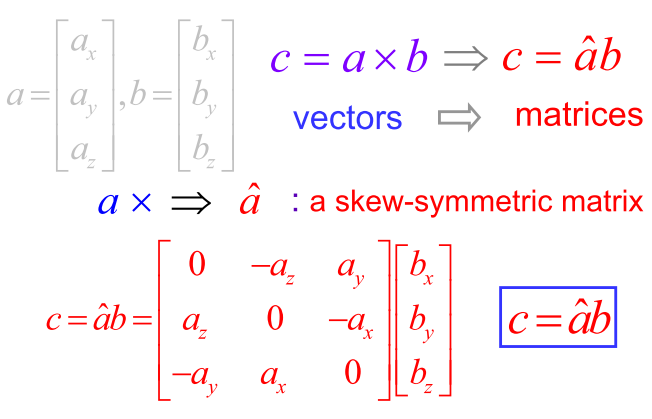
\includegraphics[height=6cm,width=1\textwidth,keepaspectratio]{image26.png}
            \label{fig:image26}
        \end{figure}
    \end{frame}
    
    \begin{frame}[t]{Cross product}
    \framesubtitle{Geometrical representation}
    \begin{columns}[T,onlytextwidth]
        \begin{column}{0.49\textwidth}
            \flushright
            $||A \times B||=||A||||B|| sin\alpha$\\
            $||A \times B||$ - area\\
            $||A||$ - length of the vector  
        \end{column}
        \begin{column}{0.49\textwidth}
            \begin{figure}[H]
                \centering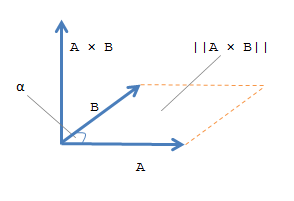
\includegraphics[height=6cm,width=1\textwidth,keepaspectratio]{image37.png}
        \end{figure}
        \end{column}
    \end{columns}
        
    \end{frame}
    
    \begin{frame}[t]{Change the coordinate frame}
    \framesubtitle{Classic way}
        \begin{figure}[H]
            \centering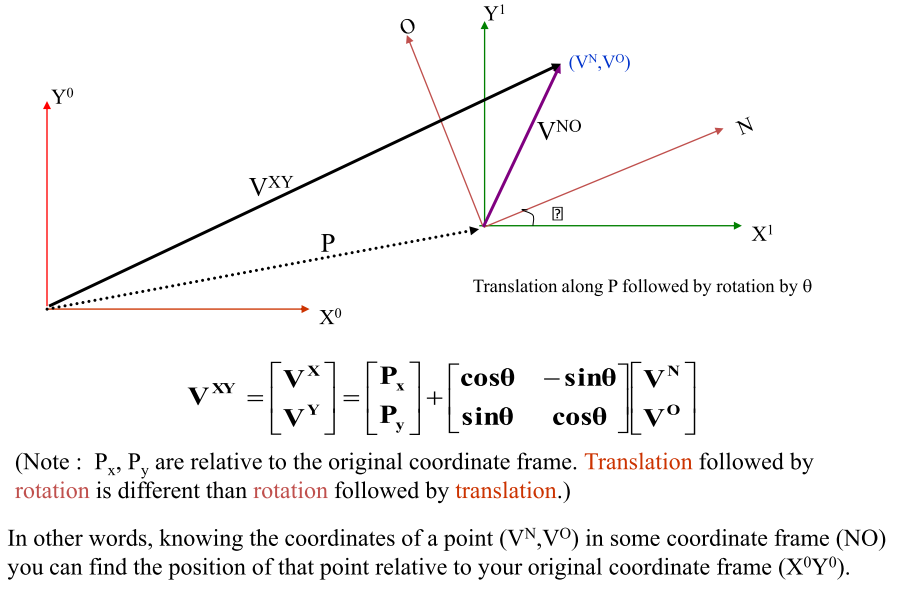
\includegraphics[height=6cm,width=1\textwidth,keepaspectratio]{image28.png}
            \label{fig:image28}
        \end{figure}
    \end{frame}
    
    \begin{frame}[t]{Change the coordinate frame}
    \framesubtitle{Homogeneous representation}
        \begin{figure}[H]
            \centering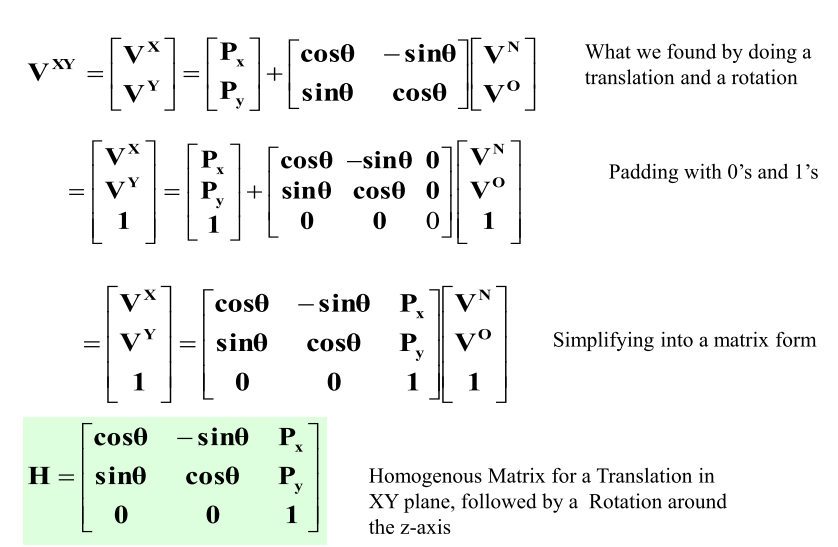
\includegraphics[height=6cm,width=1\textwidth,keepaspectratio]{image34.png}
            \label{fig:image34}
        \end{figure}
    \end{frame}
    
    \begin{frame}[t]{Change the coordinate frame}
    \framesubtitle{Case studies}
        \begin{figure}[H]
            \begin{subfigure}{1\textwidth}
                \centering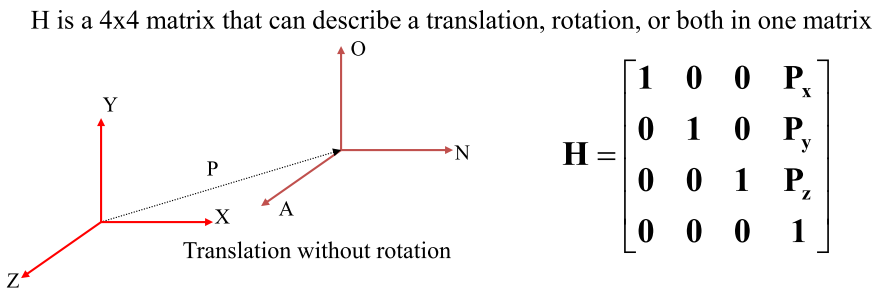
\includegraphics[height=0.35\textheight,keepaspectratio]{image33.png}
                \label{fig:image33}
            \end{subfigure}
            \begin{subfigure}{1\textwidth}
                \centering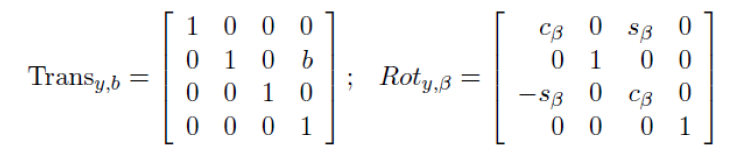
\includegraphics[height=0.34\textheight,keepaspectratio]{image29.png}
                \label{fig:image29}
            \end{subfigure}
        \end{figure}
    \end{frame}

    \begin{frame}[t]{Find a particular coordinate on the line}
    \framesubtitle{}
        \begin{columns}[c,onlytextwidth]
            \begin{column}{0.39\textwidth}
                $A,\ B$ coordinates and $|AC|$ are given: $\vec{AC}$ we want to find.
                $$\vec{AC} = \vec{A} + |AC|\frac{\vec{AB}}{\|AB\|}$$
            \end{column}
            \begin{column}{0.59\textwidth}
                \begin{figure}[H]
                    \centering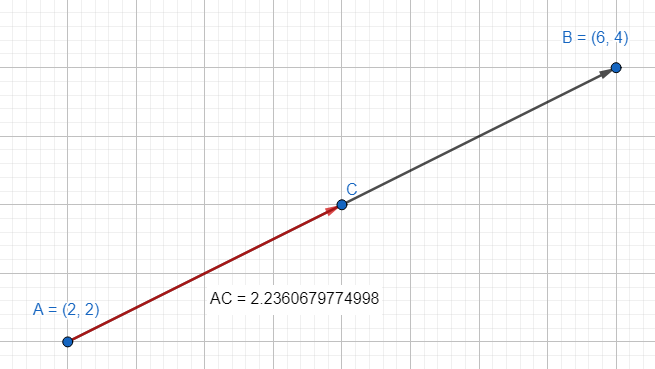
\includegraphics[height=6cm,width=1\textwidth,keepaspectratio]{exx.png}
                \end{figure}
            \end{column}
        \end{columns}
    \end{frame}

\section*{Motion representation}

\begin{frame}[t]{Formulas}
    \footnotesize
    $y = y(x)$ -- trajectory in geometry space (can be called as equation of the path)

    \centering\textbf{Forms}
    \vspace{-0.3cm}
    \begin{multicols}{3}
    \begin{enumerate}
        \footnotesize
        \item Radius vector $\vec{r} = \vec{r}(t)$
        \item Coordinate $\begin{matrix} x = x(t)\\y = y(t)\\z = z(t)\end{matrix}$
        \item Natural (arc length) $\sigma = \sigma(t)$
    \end{enumerate}
    \end{multicols}
    \vspace{-0.3cm}
    \begin{columns}[T,onlytextwidth]
        \begin{column}{0.42\textwidth}
        % \vspace{1 cm}
        \textbf{Transformations (general)}
        \begin{itemize}
            \footnotesize
            \item $2 \rightarrow 1$; $\vec{r} = \begin{bmatrix}x(t)\\y(t)\\z(t)\end{bmatrix} = x\vec{i} + y\vec{j} + z\vec{k}$
            \item $1 \rightarrow 2$; $\begin{matrix} x\\ y\\ z \end{matrix} = \begin{bmatrix}
                \cos(\alpha_{rx})\vec{r}\\
                \cos(\alpha_{ry})\vec{r}\\
                \cos(\alpha_{rz})\vec{r} 
            \end{bmatrix}$
           \item $2 \rightarrow 3$; $\sigma(t)=\int \limits _{0}^{t}{\sqrt {\dot{x}^2 + \dot{y}^2 + \dot{z}^2}}dt$ -- useless without knowing trajectory. Also, you are losing signs. \href{https://youtu.be/Hfn0Oj\_METo?si=omTZDwwpof7N9uwd}{More Info}.
        \end{itemize}
        
    \end{column}
        \begin{column}{0.60\textwidth}
        \textbf{Transformations (planar)}
        \vspace{-0.3cm}
        \begin{multicols}{2}
            \begin{itemize}
                \footnotesize
                \item $2 \rightarrow 1$; $\vec{r} = \begin{bmatrix}x(t)\\y(t)\\\end{bmatrix} = x\vec{i} + y\vec{j}$
                \item $1 \rightarrow 2$; $\begin{matrix} x\\ y\end{matrix} = \begin{bmatrix}
            cos(\alpha_{rx})\vec{r}\\
            cos(\alpha_{ry})\vec{r}\\\end{bmatrix}$
            \end{itemize}
        \end{multicols}
        \vspace{-0.3cm}
        \begin{itemize}
            \footnotesize
           \item $2 \rightarrow 3$; $\sigma(t)=\int \limits _{0}^{t}{\sqrt {\dot{x}^2 + \dot{y}^2}}dt$ -- in practice, useless without knowing trajectory.
           \item $1(2) \rightarrow y(x) \rightarrow \sigma(x)$; $\sigma(x)=\int \limits _{a}^{b}{\sqrt {1+(y'(x))^{2}}}dx$ works if $y$ is unique for each $x$
           \item $\sigma(x) \rightarrow y(x) \rightarrow 1(2)$; $\sigma_{cur} - \sigma(x) =0$.\\ Can be solved, using numerical optimization or brute force. \href{https://en.wikipedia.org/wiki/Differentiable\_curve\#Length\_and\_natural\_parametrization}{Info}.
           \end{itemize}
        \end{column}
        \end{columns}
    \end{frame}

    \begin{frame}[t]{Linear component of rigid body motion}
        \footnotesize
        \begin{columns}[T,onlytextwidth]
            \begin{column}{0.49\textwidth}
                \textbf{Linear part} \\
        Position type -- 1 = $\vec{r}$ \\
        Velocity type -- 1 = $\vec{V}$, Speed =  $|\vec{V}|$ \\        
        $\vec{V} = \frac{\mathrm{d} \vec{r}}{\mathrm{d} t} = \dot{x}\vec{i} + \dot{y}\vec{j} + \dot{z}\vec{k} = \dot{\sigma}\vec{\tau} $ \\ 
        Velocity is always tangent to the trajectory function \\
        Path function is $f$ \\
        $y = f'(x)(x-x_{cur})+f(x_{cur})$ --- easy to convert to $\vec{\tau}$ \\
        Acceleration types -- 2: tangent and normal = $\vec{a}_{\tau},\ \vec{a}_{n}$ \\
        $\vec{a} = \ddot{x}\vec{i} + \ddot{y}\vec{j} + \ddot{z}\vec{k} = \vec{a}_{\tau} + \vec{a}_{n} $\\
        $\vec{a}_{\tau} = \ddot{\sigma} \vec{\tau} = \frac{\vec{a} \cdot \vec{V}}{V} \vec{\tau}$ \\
        $\vec{a}_{n} = \frac{\dot{\sigma}^2}{\rho}\vec{n} =\frac{|\vec{a} \times \vec{V}|}{V}\vec{n}$\\
        $\rho = \frac{1}{\kappa}$, where $\kappa$ is curvature \\        
        $\kappa (x)=\frac {|f''|}{({\sqrt {1+f'^{2}}})^{3}}$
            \end{column}
        \end{columns}
        
                \end{frame}

\section*{Particle kinematics}

\begin{frame}[t]{Task 1 (mine): solution in subfolder "solution"}
    \framesubtitle{}

    \begin{columns}[T,onlytextwidth]
        \begin{column}{0.55\textwidth}
            The point $M$ motion is given in the following form:

            $ \left\{\begin{matrix*}[l]
            x=2t\\ 
            y = t^2
            \end{matrix*}\right.$
            
            When $t = 1$ sec, the goal is to find:
            \begin{enumerate}
                \item $y(x)$ --- trajectory;
                \item $\vec{v}$ --- velocity (magnitude and direction);
                \item $\vec{a}$ --- acceleration (magnitude and direction);
                \item $a_n,\ a_\tau$ --- normal and tangent acceleration;
                \item $\rho$ --- radius of curvature. 
            \end{enumerate}
            % \bigskip
            \textit{Answer}: $y(x) \rightarrow y=\frac{x^2}{4},\ \vec{v} = 2\vec{i} + 2\vec{j},\ \vec{a}=2\vec{j},\ a_n=\sqrt{2},\ a_\tau = \sqrt{2},\ \rho=5.64$
        \end{column}
        \begin{column}{0.44\textwidth}
            \begin{figure}[H]
                \centering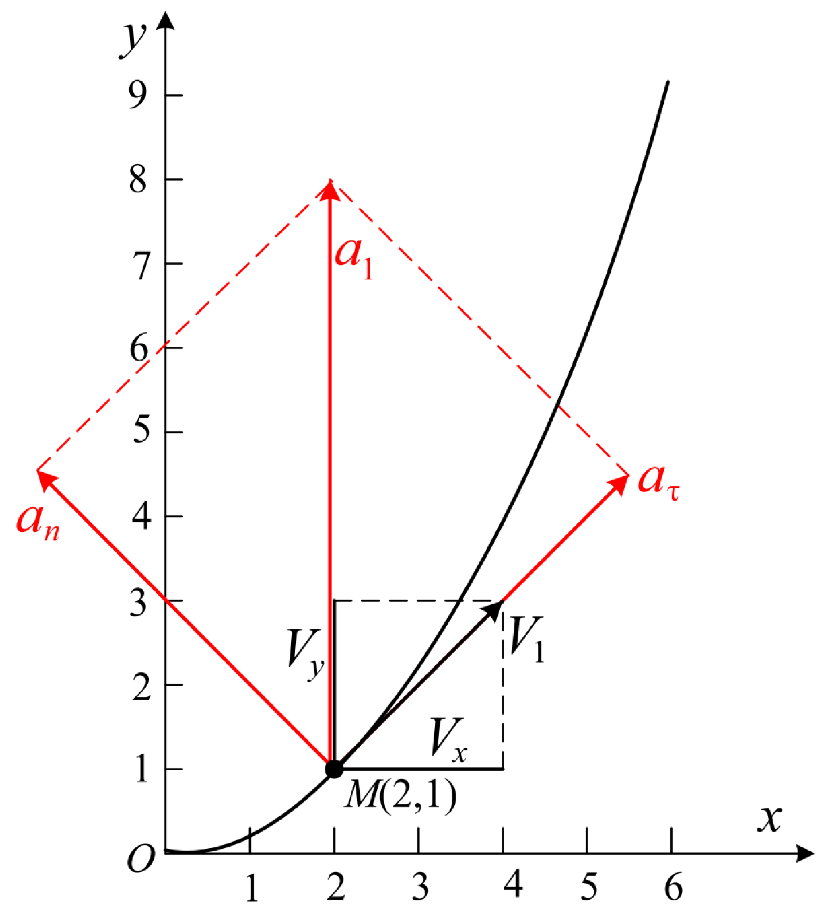
\includegraphics[height=6cm,width=1\textwidth,keepaspectratio]{image36.png}
            \end{figure}
        \end{column}
    \end{columns}

    \end{frame}
    
    \begin{frame}[t]{Task 2 (yours): M (rus) 12.15
        }
    \framesubtitle{}
        \begin{figure}[H]
            \centering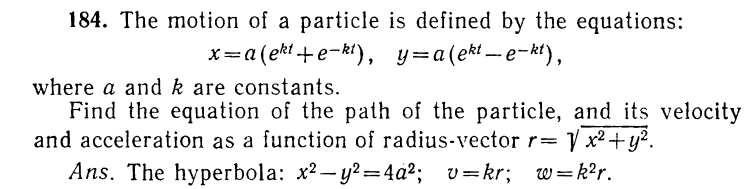
\includegraphics[height=6cm,width=1\textwidth,keepaspectratio]{image41.png}
            \label{fig:image41}
        \end{figure}
        \alert{\textit{Hint}: you should eliminate $t$, for it, take $x,\ y$ in power of 2 and think}
    \end{frame}
    
    \begin{frame}[t]{Task 3 (yours): M (rus) 12.23
        }
    \framesubtitle{}
        \begin{figure}[H]
            \centering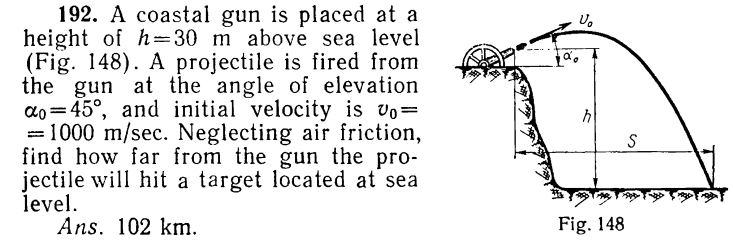
\includegraphics[height=6cm,width=1\textwidth,keepaspectratio]{image42.png}
            \label{fig:image42}
        \end{figure}
    \end{frame}

\fbckg{fibeamer/figs/last_page.png}
\frame[plain]{}
\fbckg{fibeamer/figs/common.png}

\end{document}

